\documentclass{sig-alt-release2}
\usepackage{url}
\usepackage{color}
\usepackage{graphics,graphicx}

\usepackage{epsfig}
\usepackage{epstopdf}
\usepackage{amsfonts}

\usepackage{colortbl}
\usepackage{multirow}
\usepackage{booktabs}
\usepackage{ifthen}  
\usepackage{placeins}

\begin{document}
\newcommand{\todo}[1]{\textcolor{red}{#1}}
\def\newblock{\hskip .11em plus .33em minus .07em}

\conferenceinfo{DIM3} {2012, Glasgow, UK} 
\CopyrightYear{2012}
\clubpenalty = 10000
\widowpenalty = 10000

\title{Popcorn \-- the Film Search Engine and Reviewing Application}

\numberofauthors{5}
\author{
\alignauthor
Jessica Bell, Marco Sarconi, Hristo Georgiev, Xun Zhang, David McBrierty\\
	   \affaddr{Group D}
      \affaddr{Dim3}
      \affaddr{}
             \email{\{0807335b, 0806240h, 1003619g, 1105765z, 0502862m\}@student.glasgow.ac.uk }
}
\maketitle

\begin{abstract}
Popcorn is a multimedia search mash-up. It is designed to provide a simple interface with reliance on Django and PuppyIR framework, letting users search for films, view information about the films and rate and write reviews for them.

The backend database of films is derived from IMDb \cite{imdb} using a Python script IMDbPY \cite{imdbpy}, however due to limitations of the project in terms of scale, a simulation has been implemented instead to reduce the database size.

The final implementation is not the complete set of possibly functionality for the project, and there are many more ideas and concepts as to how to develop Popcorn further in the future.

\end{abstract}

\section{Aim of Application}
Popcorn is a search engine based web application for films, that provides results with collated information on the selected film and the ability for registered users to review the film. This uses the PuppyIR Framework \cite{puppyir} to bring information together from many other web services, such as IMDb \cite{imdb} for the film details and YouTube \cite{youtube} for trailers. 
 
The goal of the design is to provide a useful and intuitive application, that satisfies the user's query about a film, and allows them to easily give their opinion through the review feature. 
  
The must-have requirements are displayed in the user matrix (Table \ref{usermatrix}) below, with the columns indicating the functionality available to the two user groups of logged in (registered) and not logged in (guest) users.

\begin{table}[h]
\scalebox{0.8}{
\begin{tabular}{| l | c | c |}
\hline
& Guest & Registered \\
\hline
Search films by title, actor, genre, keyword & \checkmark & \checkmark \\
\hline
View recent user past searches & \checkmark & \checkmark \\
\hline
See overall most viewed films & \checkmark & \checkmark \\
\hline
Produce random film result & \checkmark & \checkmark \\
\hline
View specific film information & \checkmark & \checkmark \\
\hline
Rate film search results & \checkmark & \checkmark \\
\hline
Look at other user reviews & \checkmark & \checkmark \\
\hline
Review films & & \checkmark \\
\hline
\end{tabular}
}
\caption{User needs matrix}
\label{usermatrix}
\end{table}

If time allows, the would-like requirements are for users to be able to:
\begin{itemize}
\item find out where they can buy the film or see in the cinema
\item rate or comment on other users' reviews
\item view films recommended for them by their past interactions with the application.
\end{itemize}
However the must-have requirements should be sufficient for the time the team has to develop the application.


The scope of the application is wide enough for the basic functionality of providing film information and reviews, but could be extended to provide more use with recommendations. The design goals may be somewhat ambitious considering the constraints, but with good team work should be manageable. The application is fairly complex, as it will be using several different APIs to get the search result information, requires several databases to be managed, and will implement a log in feature. The distribution of the application is most appropriate across the web, as it is one of the primary sources of information that people go to when they have a query, and films are increasingly connected with the web as television and films become more widely distributed over it.


\section{Client Interface}
The wireframes and descriptions of the user interface are included in the appendix (see Figures 1, 2 and 3). Two user personas can be imagined in the different ways to use the site. 

The first example would be Fred, who has just come home from work and would like to spend his evening watching a film, but he has no thought's as to what, and would like to browse some options. His usage of the site would be:

\begin{itemize}
\item Opens Popcorn's main page in the browser
\item Sees the random film generator feature on the bottom of the pages, and takes a chance in clicking on it
\item Reads through the returned film description page, and decides it doesn't interest him
\item Enters his preferred genre 'sci-fi' into the search box at the top of the page
\item Browses through the returned results, and clicks on the 'Like' feature where he sees an actor or description that takes his interest
\item Selects one of his 'Liked Films' from the list formed on the left navigation bar
\item Watches the trailer of the film on it's description page, and decides that it's the film he wishes to watch for his evening's entertainment
\end{itemize}

The second example would be Rebecca, a film student who watches a lot films for her course, and likes to give her opinion on them after watching, and see other people's reviews to inspire her for her next seminar. Her usage of the site would be:

\begin{itemize}
\item Opens the Popcorn main page
\item Logs in with her already registered username and password in the top right box
\item Searches for a specific film title
\item Finds the film in the results list
\item Clicks it to be taken to the film description page
\item Goes straight to reading the other user's reviews at the bottom of the page
\item Clicks the create review button and enters her opinion in the text box
\item Reads through her review, and as she's happy with it, clicks the submit button 
\end{itemize}
 
This demonstrates several dynamic components included on the user interface amongst many, such as the quick rating buttons, buttons to remove results from the past searches box, liked films box and from the results list, and the moveable and resizeable information boxes on the film information pages. This will help the user to arrange the information on the page as suits them best. The PuppyIR framework and other applications built from it such as MaSe, support this rearrangement of components in the client browser, so this can be used to implement this feature in the application. The other dynamic components can be supported using XML and JQuery.
 
The user interface is designed to be visually appealing, intuitive and simple to use, so that the user can complete their required task easily and enjoy it. On the client side, the application will be implemented using XHTML and CSS will be used to display the information, in addition to the dynamic components already mentioned, which are also beneficial in providing a separation of concerns between the structure and the style of the application.

\newpage
\section{Application Architecture}

\subsection{System Architecture}
\begin{figure}[h]
\centering
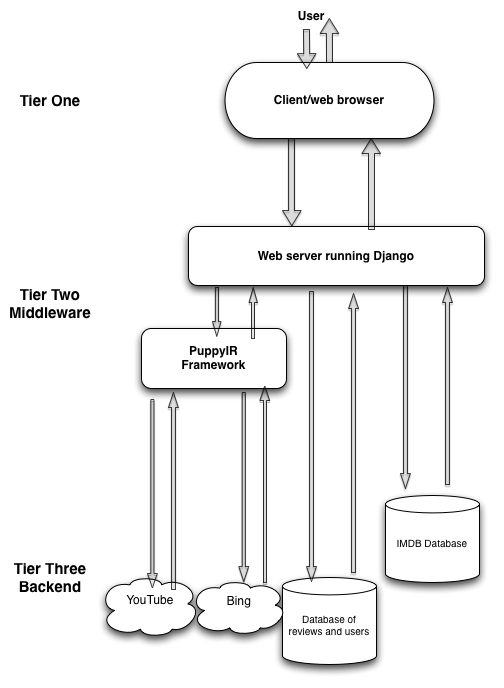
\includegraphics[scale=0.475]{tier.png}
\caption{N-Tier Architecture Diagram}
\label{architecture}
\end{figure}

Figure \ref{architecture} shows the architecture diagram that was followed in creating the system structure.
 
\subsubsection*{Tier 1: The client}
 
The client - a web browser - displays the front end of the web service to the user, allowing them to view and interact with the service without knowledge of the middleware and backend. The browser visualises the information in a user friendly form via XHTML and CSS. At this stage no specific style sheet will be created for mobile web browsers and as such the user experience may be impaired on a mobile device. 
 
\subsubsection*{Tier 2: Server}
 
The Server Tier receives queries from the client and takes required action to search relevant search services to service the user. User log in details are fetched from the Database in Tier 3, These preferences include which services to use in the search. in order to allow the user to write reviews. Results from the different backend services are prepared by this tier for presentation by the client. 
 
This tier is represented by a server running Django, it handles all the requests from the client forwarding them to the relevant backend service or to the PuppyIR framework which then carries out a web search and returns the results to the Django server. The server then deals with the various responses, processing them for display to the client. 
 
\subsubsection*{Tier 3: Database and APIs}
 
Our own Sqlite database, managed by the Django server in Tier 2, stores Popcorn's users and their credentials as well as reviews written by the users. It also stores data about each film- a unique ID corresponding to the IMDb's movieID, the number of times this movie has been selected, a rating and the number of times this movie has been 'liked'. 
 
Film data is gathered from the IMDb using IMDbPY - a Python service for searching the IMDb database. Other information about the film is collected through search services such as 'Bing' and 'YouTube' which interface with PuppyIR. 
 
\subsection{Data Model}

\begin{figure}[h]
\centering
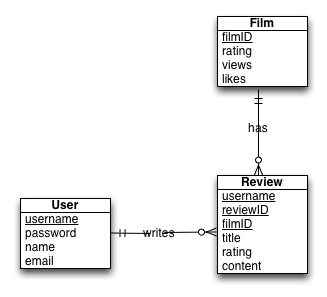
\includegraphics[scale=0.6]{erdiagram.png}
\caption{Data Model Diagram}
\label{datamodel}
\end{figure}
 
The data model, as shown in Figure \ref{datamodel} contains three tables: user, film and review. 
 
\subsubsection*{User}
Used to store log-in credentials of users and email address for possible future enhancements such as a weekly e-mail recommending films. Although it is not necessary to login to use the service, the user must be a member of the site in order to write reviews. This decision was taken to help minimise spam or abuse of the review feature. We felt users who were keen to write reviews would not mind the minor inconvenience of setting up an account. Moreover, additional benefits could be offered like member ratings. 

\subsubsection*{Film}
This table stores the number of likes a film has received and the number times it has been viewed and a rating. The rating is calculated by bringing together several different sources - the original rating taken from the IMDb, the ratings given by registered users in reviews, and the likes and dislikes given by all users. These can be averaged together with different weightings, for example giving the IMDb rating heavier weighting during the initial usage of the site, then as more reviews are gathered, giving that a higher precedence. The likes and dislikes may be less trustworthy as they are given by anonymous users and not able to be moderated, so this can be given a lower weighting.

The table also stores a unique filmID which corresponds to the movieID from IMDb's film database. This means that we do not need to store all film data such as actors, genres, plot listings etc. Instead, we can link our film ratings and other features with the data pulled from IMDb. 
 
\subsubsection*{Review}
This stores review data entered by the users. Each review is linked to a user (via userID) and to a film (by filmID), which all together form the table's primary key. The review contains the main body, a title, numerical rating for the film, and statistics about the number of users (both anonymous and registered) who have found it useful.


\subsection{Backend Services}
 
 
\subsubsection*{PuppyIR }
 
PuppyIR is a search framework, funded by the European Union, which provides tools to allow creation of search engines for children. \cite{puppyir}
 
Popcorn will utilize PuppyIR to provide a simple means of searching YouTube and Bing for movie information and trailers. It will also provide us added functionality such as query logging,and query suggestions which will cut our development time. PuppyIR is implemented in Python \cite{python} and interfaces with Django, and as such we feel it meets the needs of this project. 
 
\subsubsection*{IMDb}
 
As IMDb does not provide its own API we have decided to utilise IMDbPY.  IMDbPY is a Python package used to retrieve and manage the data of the IMDb movie database about movies, people, characters and companies. \cite{imdbpy}
It is capable of returning the results of an IMDb search in XML format. 
 
 
\subsection{Separation Of Concerns}
 
Separation of concerns is ensured by the system design, in utilising an N-Tier architecture we have ensured that each part of the system has its own responsibilities and that changes to one tier should not necessarily require changes to be made to the others. By using both XHTML and CSS we can maintain seperation of concerns in that the results or data displayed by XHTML need not be altered if we wish to change the style via CSS, to provide a mobile layout for example. 
 
\subsection{Web Framework} 
 
Although using a web application framework is not necessary, for a project of this scale it allows for rapid development, as the framework provides functionality which would otherwise have to be implemented. Having decided to utilise a web framework, we then  selected Django because it is modern and lightweight while still providing ample functionality. A further advantage of Django is that programming is done in Python with which the team are familiar, and this should save development time. Although we could have selected an alternative framework such as Java Struts, we felt that Django was the better choice and more suited to this project's needs. 
 
Using a web framework has many advantages, such as providing a structure and basis for the application and helping to enforce separation of concerns: the model-template-view pattern in Django's case. They also allow for a faster development time by implementing their own session and cookie management, providing database connectivity as well as admin services. 
 
Unfortunately web frameworks do come with some disadvantages, in that they limit choice and flexibility, and your service must conform to a structure laid out by the framework.

\section{Message Parsing}
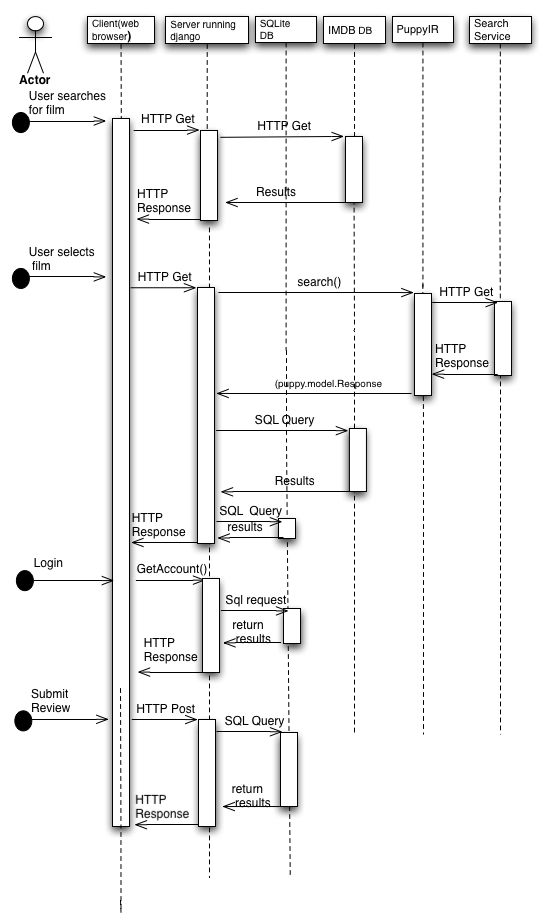
\includegraphics[scale=0.4]{seqdiagram.png}

\subsection{Format Of Messages}

\subsubsection*{HTTP GET \& Response}
The user can search for films and select films without logging in to the system. Any public user can make a HTTP request to the server. The server then returns the result as a HTTP response. For instance, the server would pass the request to IMDbPY, also using a HTTP request. The advantage of this format is that this is the  de-facto standard which is supported by all the frameworks including Django. 

\subsubsection*{XML}
The IMDbPY interface returns any result using XML. We use XML because it is supported by all the search engine APIs and Django supports XML directly. The disadvantage of XML is that it is slower to parse when compared to JSON, as JSON can be parsed using eval() using Javascript. 

\subsubsection*{SQL Query}
A SQLite database has been chosen because it is embedded in and can be managed by the Django framework. We could have used other database types such as mySQL, Oracle, etc. But since the time for development is  limited and it is beneficial to make good use of Django framework, which the team has experience in from the DIM3 course. All of the queries are Restful ones, this format was selected as it is compatible with all the search engine APIs, so it reduces the overhead associated with using multiple formats.


\section{Design Revision / Feedback}
Feedback was generally positive about the report, with marks consistently within the top two categories for every section with a choice given. It showed that the report needed some tidying up to aid understanding, and to clarify the design for the reader. This was done in several areas of the report, one example being the list of requirements being put into a user matrix and bullet points.

With the written feedback, each comment was analysed to find the cause and solution to the problems found.

These comments were particularly good at highlighting areas where more explanation was needed, for example the notation used to show the scrolling of the page in the final wireframe diagram, and also found the odd mistake that had been overlooked in the message parsing diagram. Other changes included the clarification of the user descriptions, walkthrough and message examples. These changes were easily integrated into the implementation report.

Other comments concerning system design were considered individually, and not all were thought to be right to be included. For example, the suggestion that the database components should be moved into the second tier of the architecture diagram was not taken on board, as it was felt that whilst the databases are still managed by the Django middleware server, the separation into the third tier demonstrates that the database originates from external sources, for example IMDb. However the comment raising the issue of moderation was very helpful, as it is an important area that had not yet been addressed.

\section{Implementation Notes}

\subsection*{Views}
All the main views have been implemented, along with their XHTML and CSS pages. These are the main page, results page, film description page and reviews page. They are not all connected, but are accessible through each of their URLs. Despite not all functionality having yet been implemented, the pages demonstrate, for example, where the search results would be shown and the layout of the film description page.

\subsection*{URL Mapping Schema}
The URL mapping schema has been set up as follows:
\begin{itemize}
\item {\it r'\textasciicircum popcorn\textunderscore app/ \textdollar ' } \\
to the main page: index \textunderscore with\textunderscore menu.html
\item {\it r'\textasciicircum popcorn\textunderscore app/query/ \textdollar '} \\
to the results page: query\textunderscore results.html
\item {\it r'\textasciicircum popcorn\textunderscore app/film/ \textdollar '} \\
to the film description page: view\textunderscore film.html
\item {\it r'\textasciicircum popcorn\textunderscore app/reviews/ \textdollar '} \\
to the reviews page: view\textunderscore reviews.html
\item {\it r'\textasciicircum media/(?P<path>.*)\textdollar '} \\
for retrieving media from the static folder, which must be edited in settings to the current local path of the folder
\end{itemize}

\subsection*{External Services}
It was found that using IMDbPY integrated in the application would require it to be installed onto the system being used first, and so was not possible to distribute easily in this instance. So the option was taken to use IMDbPY's additional service of creating an offline database of IMDb, which could then be managed by the Django server. As previously discussed, this database was too large to currently be of use, and was replaced by a simple simulation.

YouTube has been used as an external service for retrieving trailers, but the query functionality to do this has not yet been implemented.

Future extention of the project would see the inclusion of Bing as an external service to retrieve information about where it is possible to buy, rent or see a film in the cinema.

\subsection*{Functionality Checklist and Known Issues}
Due to team organisation issues and due to other work commitments, the functionality of the project has yet to be implemented, although with only a little more time it would be possible to integrate many of the key features into the system set up.

\subsection*{Technologies Used}
As mentioned, Django is the key framework technology used, and SQLite for the database, with PuppyIR having been set up but not currently in use in the application, and also IMDbPY not being used in this implementation, but possibly in future developments.


\section{Reflective Summary}
The team has learnt that web application requires more time than expected, a major lesson that has been learnt for the future. The framework helped our progress in allowing us to build up the base structure quickly, however we had problems with integrating the other technologies needed.

One of the major achievements is to have managed to create the huge database of IMDb locally, although it was not possible to use this in the end. This was possibly a mistake that lead to not as much of the project being implemented as we would have wished, as this aspect took up a large amount of time that we should have spent on other aspects.

\section{Summary and Future Work}
 
\subsection*{Summary}
 
This service is currently in development. On completion we hope to offer an interesting, intuitive web service based around finding films to watch and reviewing those films. The main limitations for this project are the very limited timescale and a restriction on available resources. 
 
\subsection*{Limitations}
 
The project is constrained by the small amount of time to complete the application with a relatively small team to work on it. Although many ideas have been formed about the functionality of the application, it would not be possible to implement them all in the time available. Also the project is constrained in terms of the language and tools used to create it, as the team is inexperienced in building web applications. The application will be implemented using the Django framework and PuppyIR framework, as the team has had most experience with it, and as it is requested by the course lecturer. 
 
\subsection*{Plans For Future Development}
 
Support of user ranks could be implemented. For instance: (special ranks) Site Administrator, Moderator; (ranks based on the number of reviews made) Newbie 0, New user 10, Novice 50, Active user 100, VIP user 500, Legend 1000 etc. 
 
Another feature that could be added to the project is the support of registered users being able to add comments (and 'find them useful', i.e. rate them) to reviews, thus introducing some form of hierarchy. This would give users the ability to criticise a particular review, or agree or disagree partially with it, by being more specific in the corresponding comment. 
 
Also, the film information could be made editable, i.e. maintained in a wiki style by having open discussions about the different sections of a particular set of film data. Thus, any registered (and trusted - this could be implemented by allowing only users meeting particular requirements, e.g. minimum number of reviews made, in addition to a minimum rating - which can be combined with or derived from the rank support feature) user could help improve and keep the site up-to-date. 
 
Additional film information could be added. For instance, where a particular film can be purchased (providing a list of online shopping services). 
 
Functionality that was initially discussed but decided would require too much time, would be to supply personalised film recommendations, possibly as a substitution for the random film feature on the main page. This could be based on a registered users film ratings, past searches and films viewed, or by the user entering certain preferences, and then using some form of algorithm to create a list of films to recommend. There are several methods that could be used to implement this, so research would need to be done to decide on the best way this could be achieved.

\section{Acknowledgements}
Our thanks to the lecturers and demonstrators for their comments and suggestions.

\section*{}
\begin{thebibliography}{9}
\bibitem{puppyir} Glassey R, Polajnar T and Azzopardi L 2011 PuppyIR Unleashed: A Framework for Building Child-Oriented Information Services {\it The Dutch-Belgian Information Retrieval Workshop, Amsterdam, Netherlands}\\
\bibitem{imdb} IMDb: {\it www.imdb.com}\\
\bibitem{youtube} YouTube: {\it www.youtube.com}\\
\bibitem{imdbpy} IMDbPY: {\it http://imdbpy.sourceforge.net}\\
\bibitem{python} Python: {\it www.python.org}\\
\end{thebibliography}

%\bibliographystyle{abbrv}
%\bibliography{sig-proc}

\newpage
\appendix
\section{Wireframes}

\textbf{Figure 1}\\
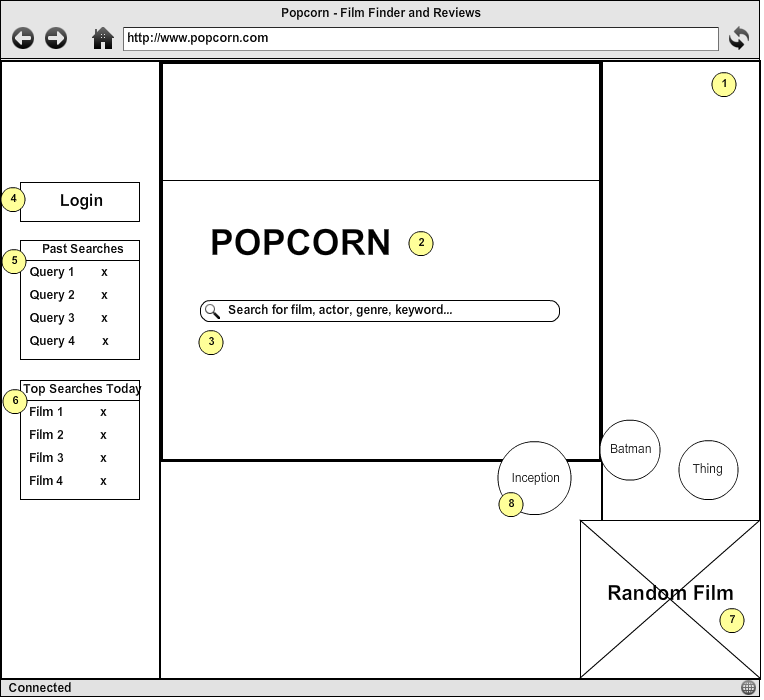
\includegraphics[scale=0.33]{wireframe1.png}\\
 
1 - Background image of cinema screen \\
2 - Logo \\
3 - Search field, with search instructions when not selected \\
4 - Log in - expands to allow entry of username, password, or registration \\
5 - If users has already searched in current session, the last searches (to a maximum of 5) are shown \\
6 - The most viewed films by all users in the last 24 hours are shown here \\
7 - An image of a popcorn box, that when clicked leads to an information page of a random film \\
8 - Images of popcorn with random film titles on, that lead to the respective film information pages\\

\newpage
\textbf{Figure 2}\\
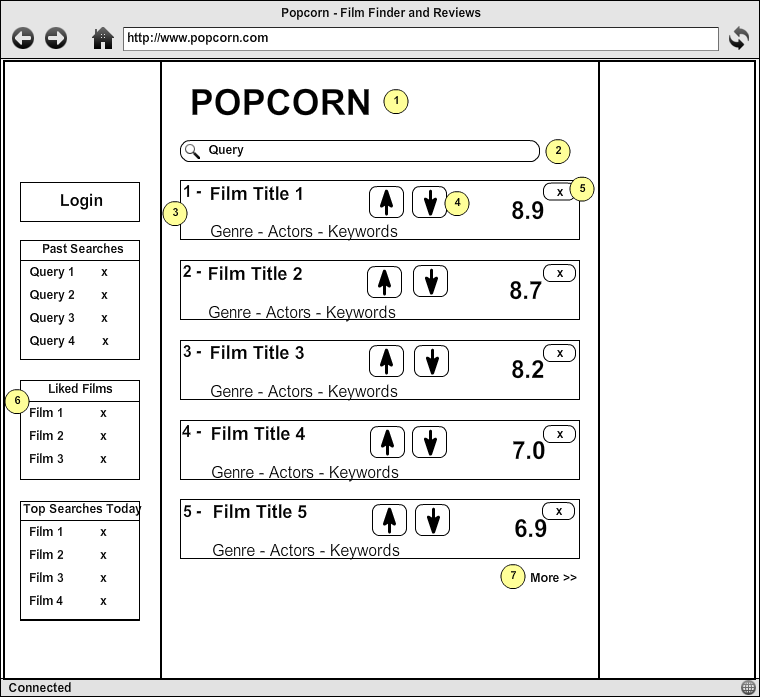
\includegraphics[scale=0.33]{wireframe2.png}\\
 
1 - Logo, links to main search page \\
2 - Search field, containing current query \\
3 - Film result with summarised information: genre, actors, keywords, rating \\
4 - Quick rating buttons - like or dislike, with liked films showing up in box 6 \\
5 - Remove result button, the result is removed and next result is added to bottom of list - the result is removed only during the current search, and would reappear when searched again \\
6 - Liked films, with x to remove like rating \\
7 - Show next 5 search results\\

\newpage
\textbf{Figure 3}\\
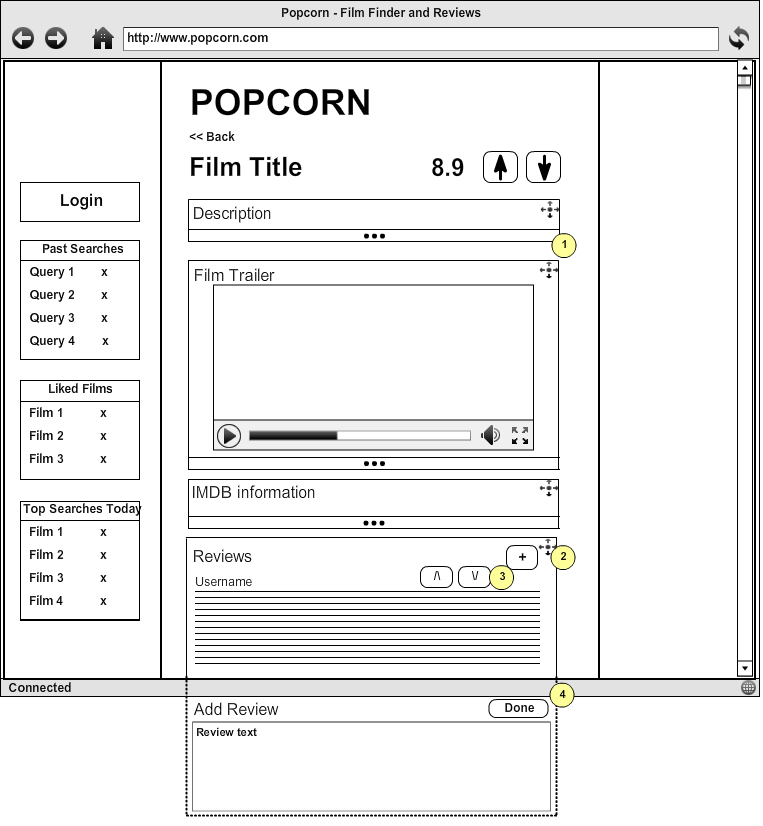
\includegraphics[scale=0.33]{wireframe3.png}
1 - Moveable, resizeable information boxes \\
2 - Reviews with add review entry at bottom of page, and add review button to jump to it \\
3 - Like and dislike quick rating buttons for individual reviews \\
4 - Create review form at bottom of page, after scrolling past all reviews or using the add review entry button at top of reviews to jump to the section\\



\end{document}
